
%(BEGIN_QUESTION)
% Copyright 2006, Tony R. Kuphaldt, released under the Creative Commons Attribution License (v 1.0)
% This means you may do almost anything with this work of mine, so long as you give me proper credit

Et trykkmåler skal vise pålagt trykk riktig over hele kalibrert område.  I dette eksemplet utsettes et manometer med område 0 til 500 PSI for fem ulike trykk i dette området, og responsen er korrekt i alle punkter:

$$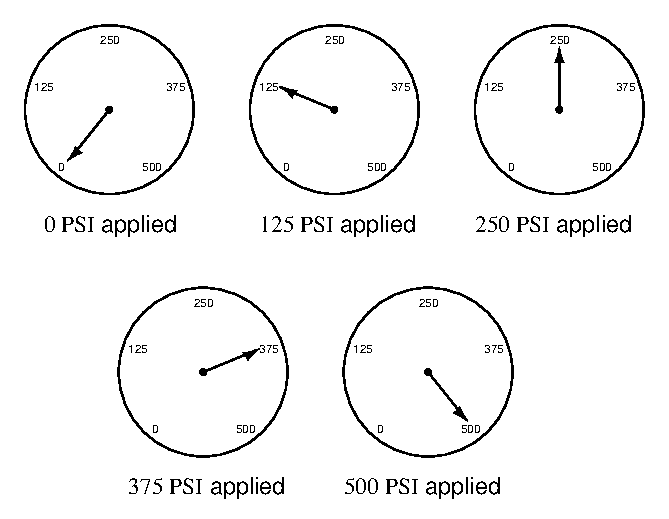
\includegraphics[width=15.5cm]{i00174x01.eps}$$

Beskriv, ved å tegne et sett med fem avlesninger som settet over, hvordan et trykkmåler som er riktig ved 0\% og 100\% av pålagt trykk -- men har et \textit{linearitetsproblem} mellom LRV- og URV-punktene -- kan reagere på de samme fem trykkene.

\vskip 10pt

Beskriv videre hvordan et bourdon-rørs trykkmåler kan justeres for linearitet.  Med andre ord: hvordan kan et ikke-lineært trykkmåler kalibreres for å bli mer lineært?

\vskip 20pt \vbox{\hrule \hbox{\strut \vrule{} {\bf Suggestions for Socratic discussion} \vrule} \hrule}

\begin{itemize}
\item{} Forklar hvordan det å bevare bade ``As-Found'' og ``As-Left'' kalibreringsdata for instrumenter som dette gor det mulig å følge kalibreringsdrift over lang tid.
\item{} Kan en linearitetsfeil korrigeres ved å justere null- og/eller span-skruer på et instrument?  Hvorfor eller hvorfor ikke?
\end{itemize}

\underbar{file i00174}
%(END_QUESTION)





%(BEGIN_ANSWER)

Her er ett eksempel på hvordan et trykkmåler kan reagere ikke-lineært på de samme fem pålagte trykkene, samtidig som det fortsatt er riktig ved LRV- og URV-punktene:

$$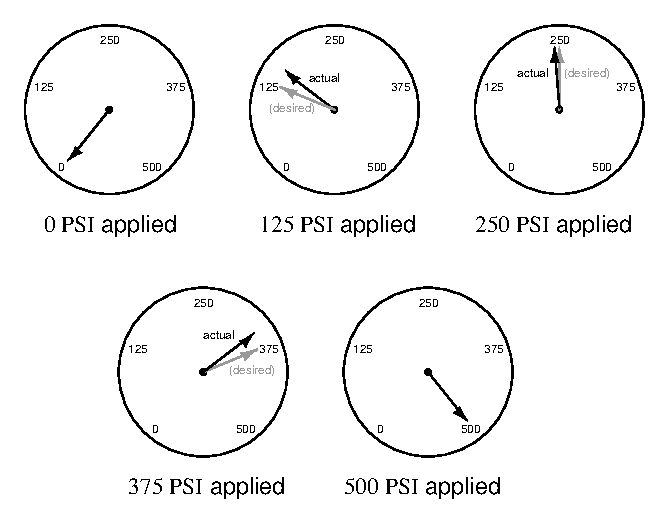
\includegraphics[width=15.5cm]{i00174x02.eps}$$

Her viser manometeret for høyt ved 25\%-punktet (125 PSI), litt for lavt ved 50\%-punktet (250 PSI), og lavt ved 75\%-punktet (375 PSI), men fortsatt riktig ved 0\% (0 PSI) og 100\% (500 PSI).

\vskip 10pt

Enhver justering som påvirker mekanismens \textit{vandringsvinkel} vil påvirke lineariteten.  Noen trykkmålermekanismer (høy kvalitet) har justerbar linklengde for å lette endring av denne vinkelen:

$$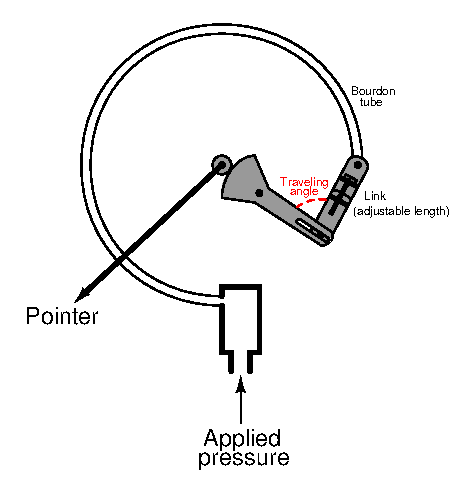
\includegraphics[width=15.5cm]{i00174x03.eps}$$

Det er god praksis å \textit{la alle vinkeljusteringer sta i fred} til alle mulige null- og spanjusteringer er gjort.  Ofte er det mulig å fa et ikke-lineært instrument innenfor toleranse i en 5-punktskalibrering kun ved null- og spanjustering.

I mange mekaniske instrumenter er en enkel linearitetskontroll å pålegge 50\% inngangssignal og sjekke link/spak-ortogonalitet (at alle linker og spaker krysser hverandre med 90$^{o}$ vinkel).

%(END_ANSWER)





%(BEGIN_NOTES)

Det bør merkes at ikke-linearitet i instrumentet ikke betyr at feilen må veksle mellom for høy og for lav avlesning.  Grunnleggende er ikke-linearitet definert som \textit{enhver} tilstand der instrumentet er riktig i (minst) to punkter, men ikke i alle punkter i kalibrert område.

Hvis manometeret var perfekt lineært, ville riktighet i to punkter nødvendigvis gi riktighet i \textit{alle} punkter.  I praksis er alle instrumenter ikke-lineære i en eller annen grad: spørsmålet er hvor ikke-lineært det kan være og fortsatt oppfylle minstekrav for total nøyaktighet.

\vskip 10pt

En praktisk anvendelse av \textit{bevisst} ikke-linearitet i et link/spak-system er Ackerman-vinkelen i bilstyring.  Dette kan være nyttig å vise for studenter for å forstå betydningen av vandringsvinkel i et mekanisk manometer.

%INDEX% Measurement, pressure: nonlinearity in pressure gauge

%(END_NOTES)
